\documentclass[11pt]{article}
%Gummi|065|=)
\usepackage[english]{babel}
\usepackage{graphicx}
\title{\textbf{Welcome to Gummi 0.6.5}}
\author{Alexander van der Mey\\
		Wei-Ning Huang\\
		Dion Timmermann}
\date{}
\begin{document}

\maketitle

\section{Handling Missing Data}

Upon first inspection of the data we see there are many missing values. This is common in datasets and can be the result of many situations- within surveys, for example, participants may have refrained from answering certain questions or stopped participating part way through a long term study into the impact of, say a new medicine. 
Missing data becomes a serious problem, however when we wish to make inferences by fitting models to the full data set and we need meaning full values in every cell of our database. 

\subsection{Omitting missing data}
The quickest way to solve the missing data problem is to omit every observation where at least one variable has a missing value.  

\begin{verbatim}  
marketing = na.omit(marketing)  
\end{verbatim}

The simplicity of this method comes a price because we lose all the information contained in any of the other variables for an observation which carries even a single missing value.


\begin{verbatim}
> sum(is.na(marketing))/dim(marketing)[1]
[1] 0.2995663
\end{verbatim}

In the case of our marketing dataset there are approximately 2600 such observations which make up about 30\% of the data. Losing so much of our data would have a significant impact on the validity of any fitted models. We need a more preservative way to deal with the missing values.

\subsection{Replacing with the predictor mode}
It is common practice when dealing with missing data to replace missing values with the mean value of the variable in question. For categorical data, such as that in our marketing data, the mode of the data performs similarly. Note that we must not fill-in/impute any values for 'Income' as this is our response variable.
The following function can be called on our marketing data set to carry out the necessary substitutions. The mode function involved has been written separately as this is not included in R by default.


\begin{verbatim}
NA_to_mode = function(m){
  for ( i in 2:14) {
    m[,i][is.na(m[,i])] = Mode(na.omit(m)[,i])
  }
  return(m)
}
\end{verbatim}

This method has the major advantage over the latter in that we dont't lose any of the information stored in data values adjacent to missing data. Implementing this method does not require a significant amount of computing time in the case of our dataset.
\\

 One potential flaw in this method is that all the missing values of a variable will be given the same value. The reason these data are missing may be significant, e.g. members of a given ethnic background may have been generally reluctant to divulge said information to a survey, this may have resulted in the majority of missing 'Ethnic' values actually belonging to people of the same given ethnicity which, crucially would not be reflected in the mode of the available “Ethnic” values.
\\

\subsection{Multiple Imputation}
To combat this potential bias, we can look at the available data fo the observations in question and base our imputations on them. For this method we will make use of the CRAN Package “mice”. This package can implement multiple techniques to predict data values depending on whether they are ordered/unordered categorical or continuous etc. Once we specify these methods, we can run the  following command

\begin{verbatim}
data(marketing)
result = (mice(marketing, m =5, me = method))
\end{verbatim}

to perform several iterations of these methods of imputation and finally update our marketing dataset with the new complete dataset.

\begin{verbatim}
marketing = complete(result,1)
\end{verbatim}

Despite the extra computation time, this method of multiple imputation is the best of the three we have investigated because it neither removes valuable information from the data nor does it assign the same value to each missing value of a given variable regardless of the available adjacent data.
\\

Having decided on our imputation method, we are now in a position to proceed to fit various models to the data with the aim of inferring which of our predictors best predict the value of 'Income'. We decide to make one last check before proceeding- to see how much of the data for each predictor we have actually imputed.



\begin{figure}[h!]
  \caption{Proportion of Missing Data.}
  \centering
    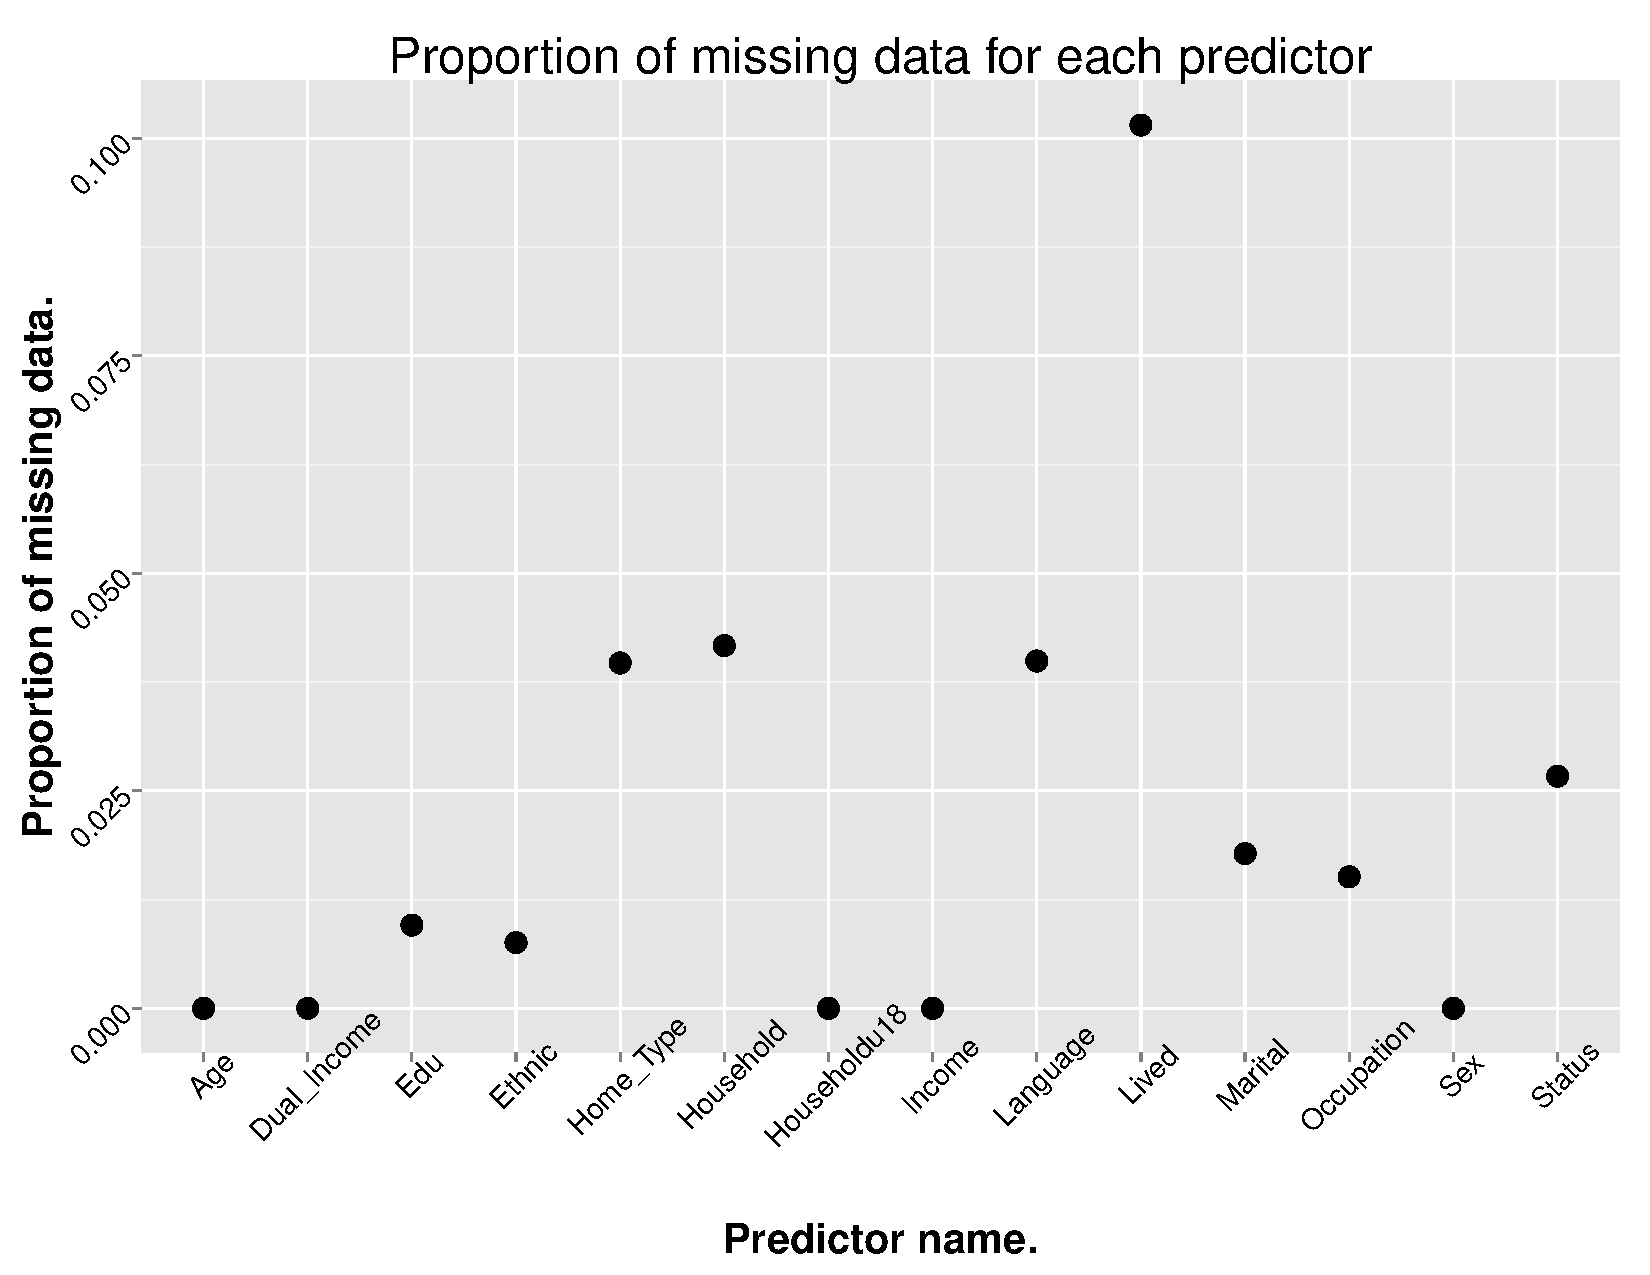
\includegraphics[width=1.0\textwidth]{HandlingMissingData/PropMissingData.pdf}
\end{figure}


One value catches our attention- the predictor 'Lived' has required 10\% of it's data to imputed. This may reflect badly on any apparent significance to this predictor later in our analysis.



\end{document}
